\section{Method}

\subsection{Research methodology}
We chose to follow the four-step method of Pólya. This method was chosen since it divides the problem into smaller, more perspicuous problems. This method allows for an iterative work process, which will produce deliverable products that can be improved on in increments. The model contains four steps: Understand the problem, Devise a plan, Implement the plan, and Evaluate and control. \\
The four-step method and its parts can be seen in figure \ref{fig:project-polya}.

\begin{figure}[ht]
	\centering 
    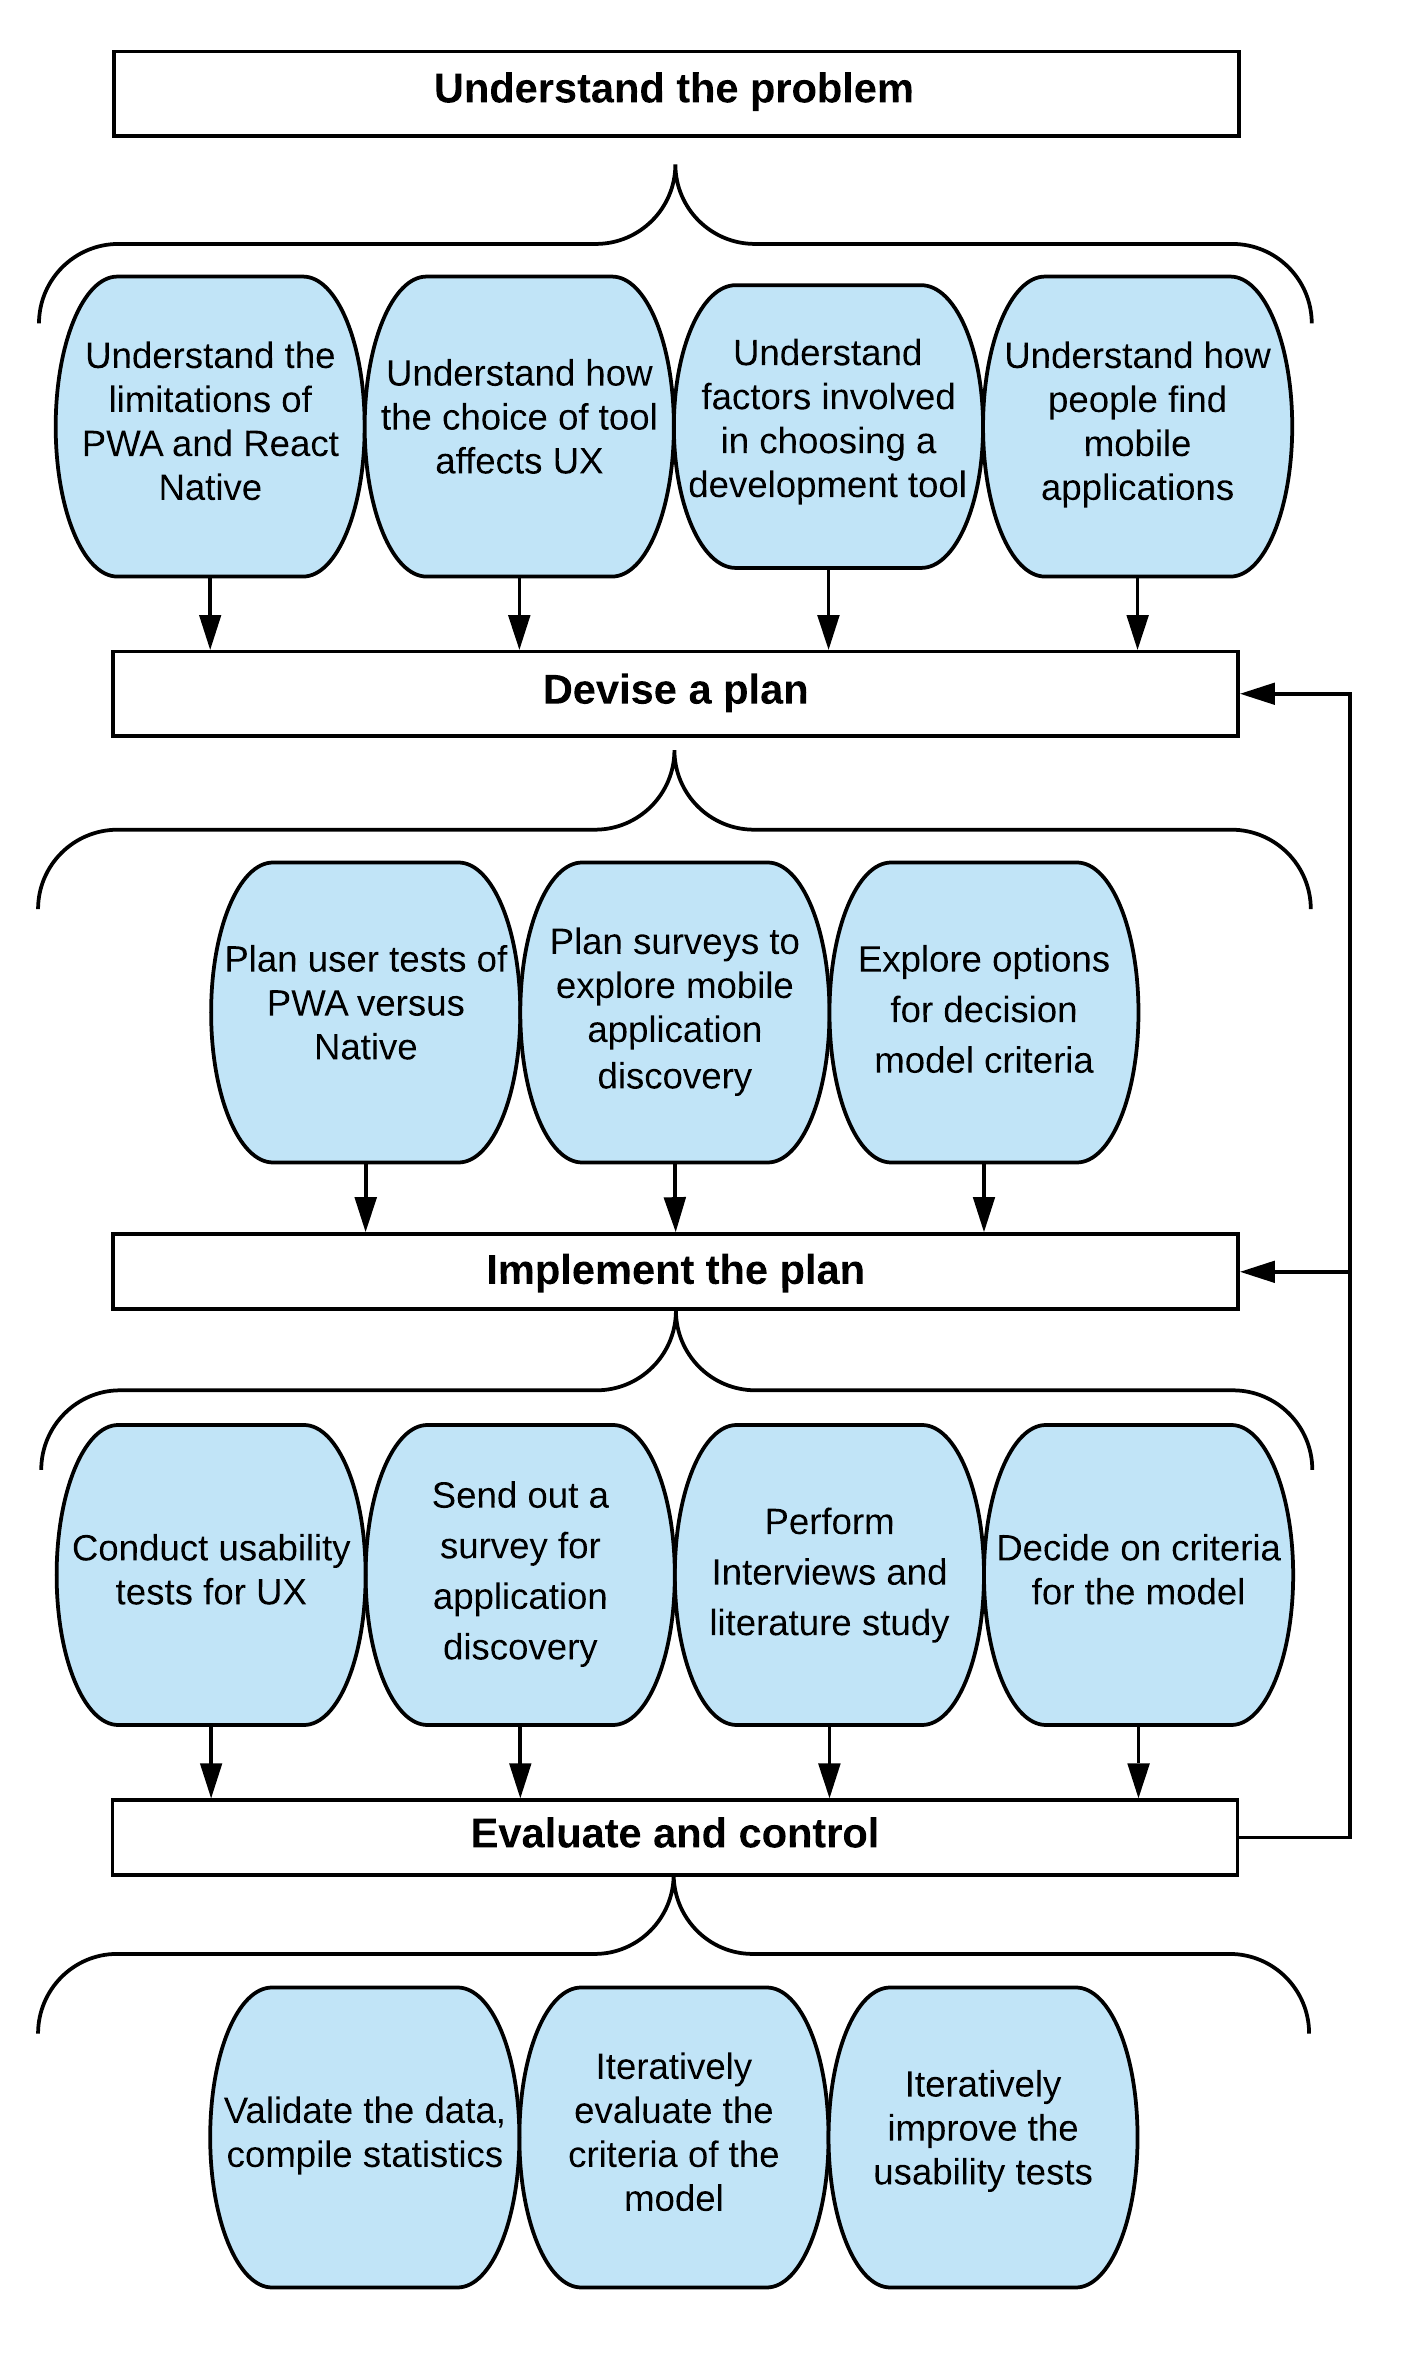
\includegraphics[width=0.6\textwidth]{img/Polya.png}
	\hfill
	\caption{\textit{Implementation of Pólya's four-step method.}}
		\label{fig:project-polya}
\end{figure}

\subsection{Project methodology}

\subsubsection{The project triangle}
The project triangle describes how the quality of the project correlates with the time, cost and scope. The cost and time of this project were predetermined, so the only mobile variable was the scope. This means that the scope of the project could have been extended or cut as needed. This could have been applied to the usability tests, as more or fewer tests could have been conducted depending on the time left. The quality of the results would have been improved if more tests had been conducted.

\begin{figure}[ht]
	\centering 
    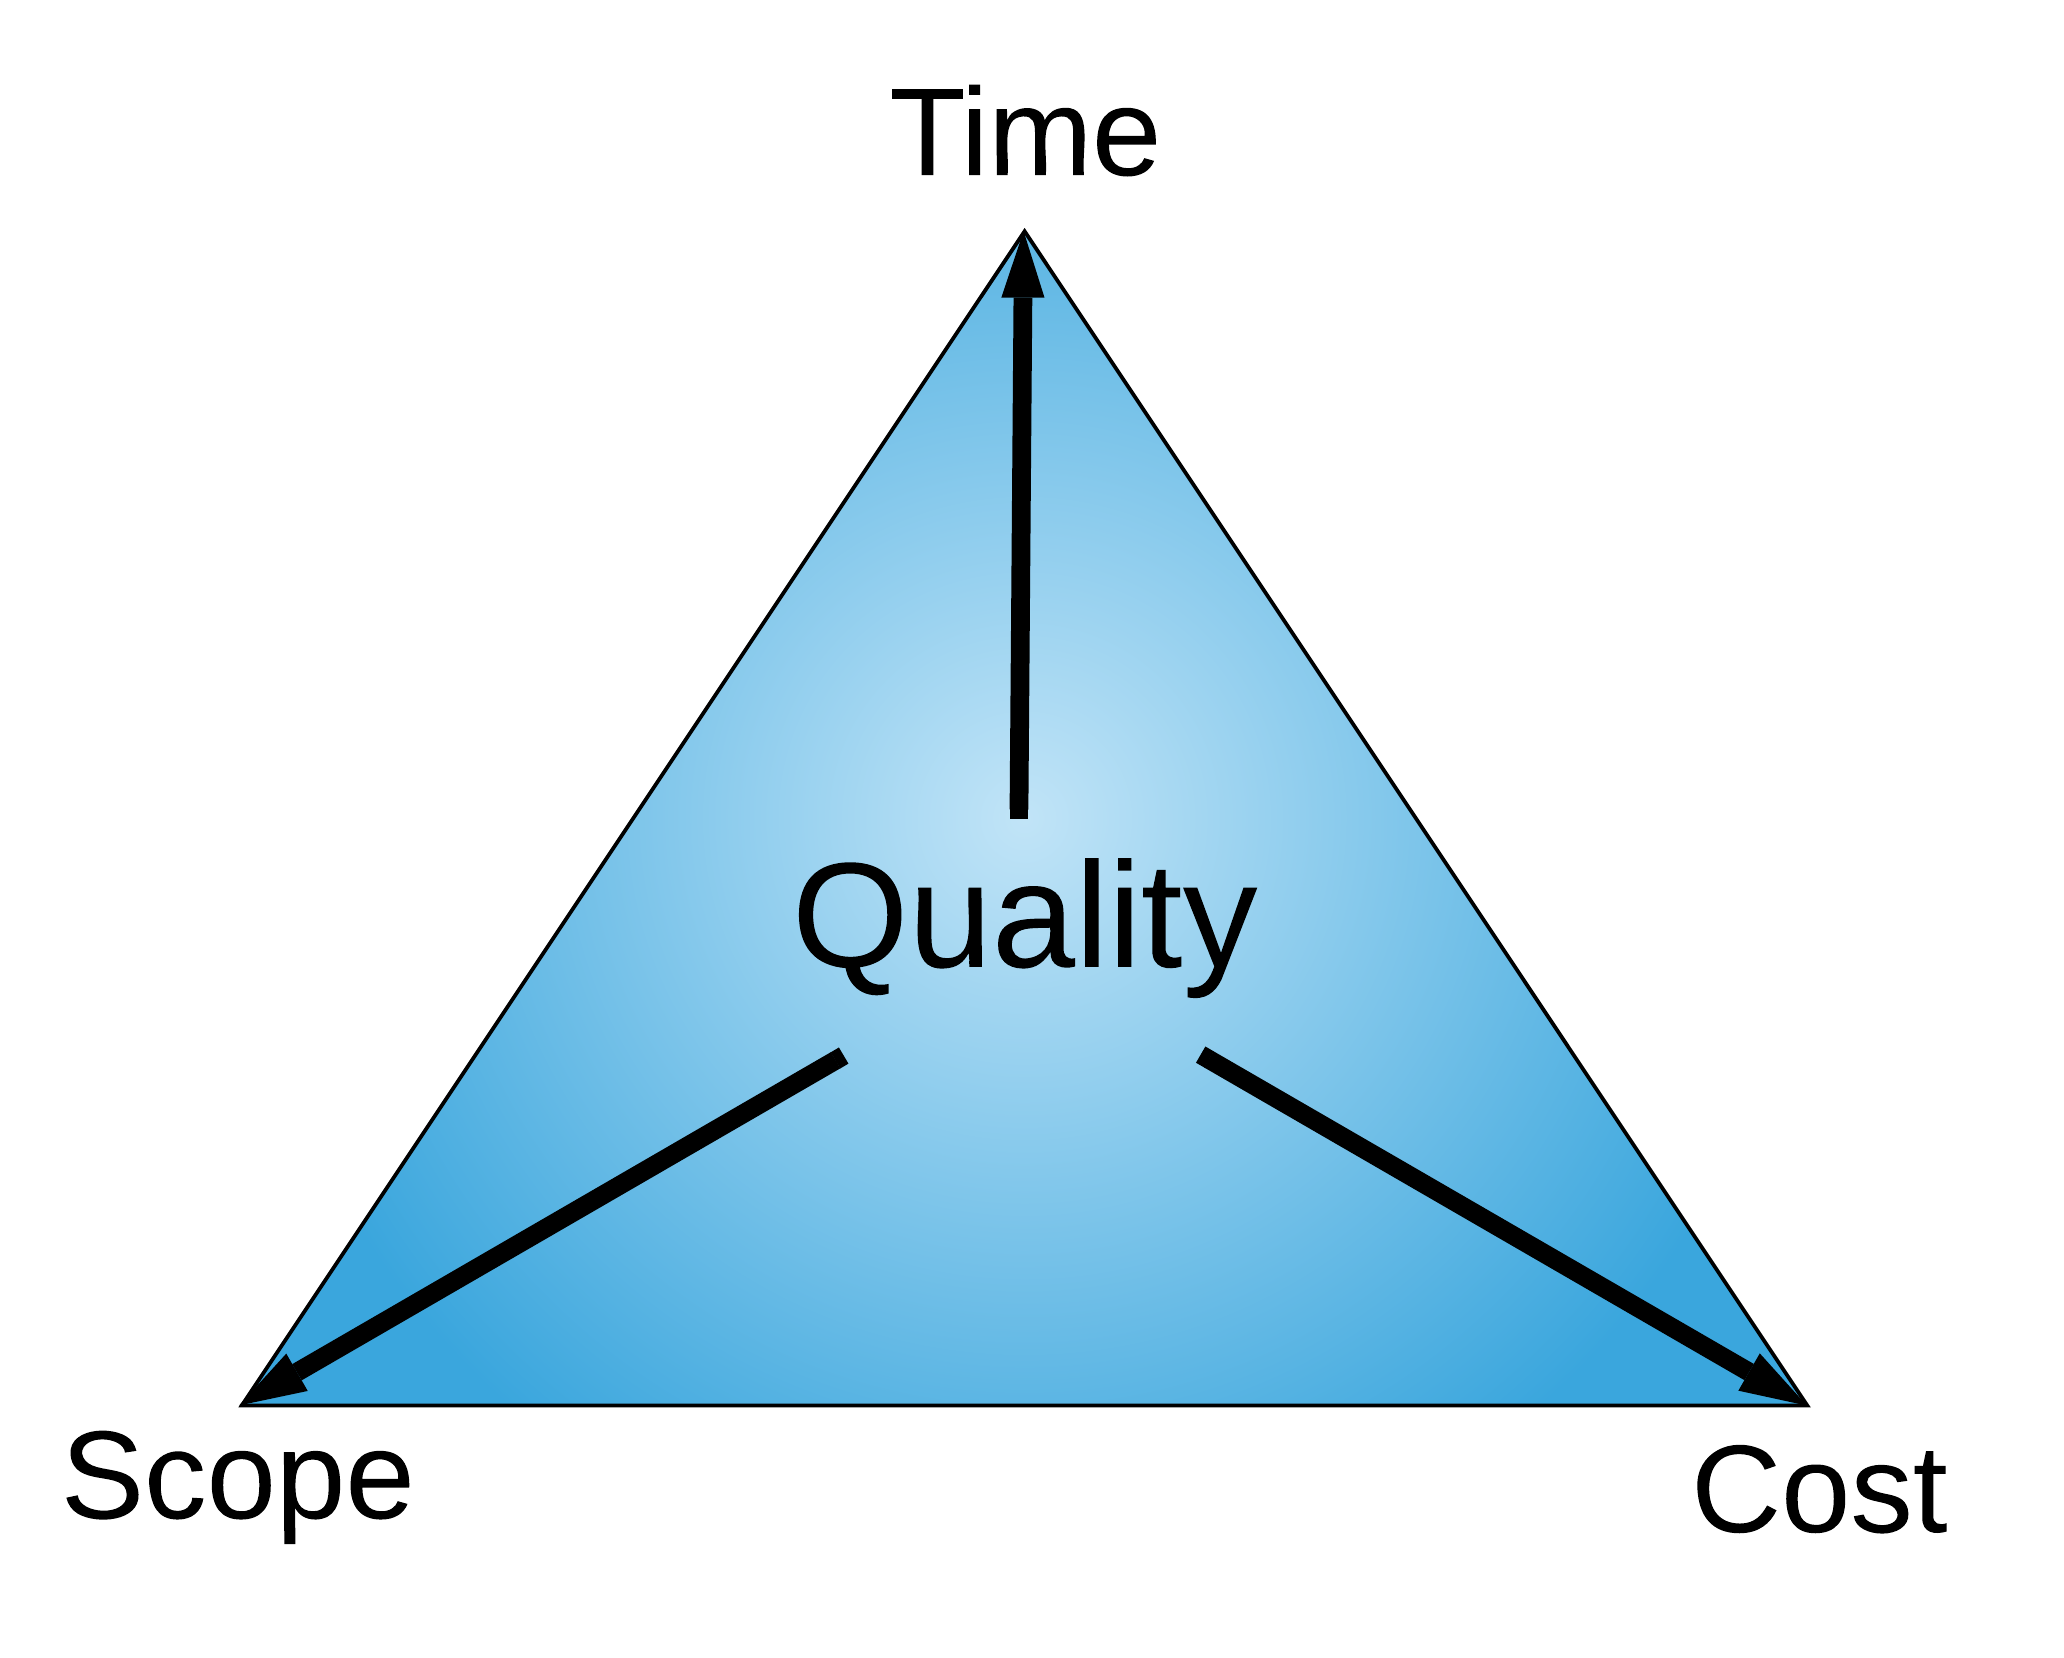
\includegraphics[width=0.6\textwidth]{img/project_triangle.png}
	\hfill
	\caption{\textit{The project triangle}}
	\label{fig:project_triangle}
\end{figure}

\subsubsection{MoSCoW}

MoSCoW is a method used to prioritize during project management. The term MoSCoW is an acronym for the four prioritization categories: Must have, Should have, Could have and Won’t have. The MoSCoW was chosen due to its ability to fraction the project into a core assignment and possible improvements. 
The MoSCoW for this project can be seen in figure  \ref{fig:MoSCoW}.

\begin{figure}[ht]
	\centering 
    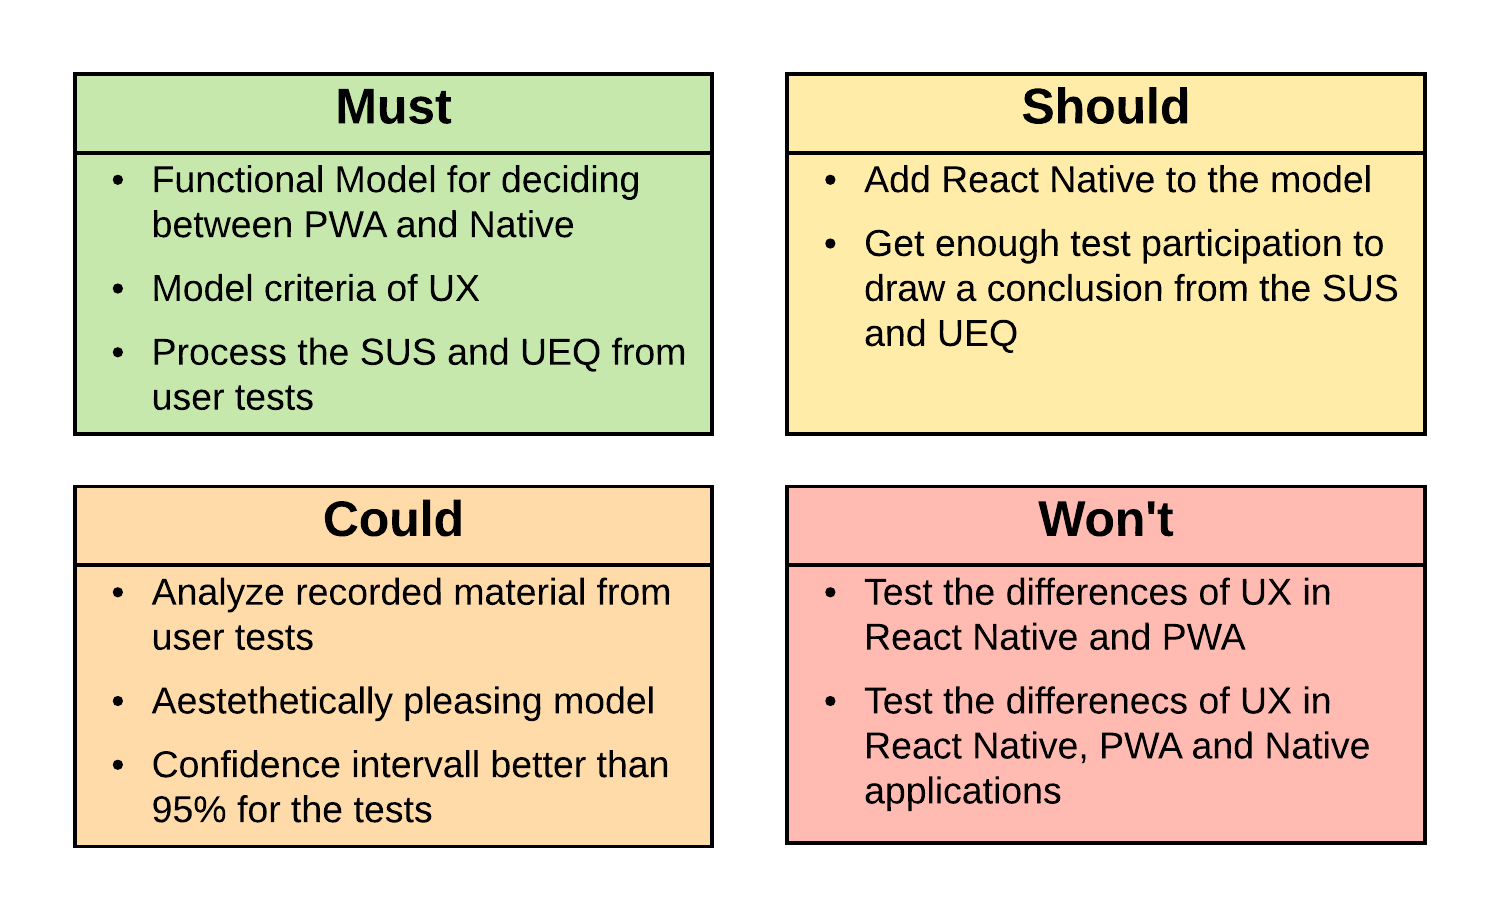
\includegraphics[width=0.9\textwidth]{img/moscow.png}
	\hfill
	\caption{\textit{MoSCoW chart of this project}}
	\label{fig:MoSCoW}
\end{figure}

\subsection{Literature Study}

To understand what differences there are between the different types of mobile applications there had to be some extensive research. Mobile applications that use more of a hybrid approach, such as PWA, tend to follow trends. This means that if the technology does not get enough attention it might go extinct. This is happening to many Javascript frameworks such as Angular according to Slagkryssaren AB. The information available on this subject is both opinion- and research-based.\\

For the MCDM, the design practices and evaluation processes are investigated. 
In order to conduct usability testing, it was a requirement that these tests should follow typical practices currently in use. This includes how to design, conduct and validate usability tests.
Typical places where information was gathered were:

\begin{itemize}
    \item Blogs, forums and similar websites
    \item Research articles and technical literature 
    \item Opinions from developers and experts within interaction design
\end{itemize}

\subsection{Case study}
Since the model was to be used by Slagkryssaren AB, the development of the model was done in close co-operation with the company’s consultants. These consultants have extensive experience in the field of developing applications and choosing application development tools. This inductive approach was more suitable than a deductive, as there is no decidedly right or wrong conclusion when choosing an application development tool.
\newline
To conduct the case study, consultants were interviewed. These interviews were to be unstructured in an attempt to get richer, more opinion-based data. A combination of planned and improvised interviews were done to answer questions emerging during the progression of the project. 

\subsection{Application usage survey}

The survey was conducted to explore two hypotheses, one of them being that people tend to find information about applications mostly on the platforms application store, rather than using web searches. The other hypothesis was that Android users tend to look for information about applications through web searches, while iPhone users tend to go to the App Store first. This was done to understand the consequences of releasing an application which can not be found on the platform’s store, which is the case for PWAs. 

\subsection{Usability testing}

The users tested two versions of the same application, Yummly \cite{Yummly}, on the same platform they normally used. One of the applications was a PWA and the other a native application. In the usability tests, both qualitative data, in the form of questions and thinking-out-loud, and quantitative data, in the form of a SUS and a UEQ, was collected. 
\newline
The subject got a list of six tasks to perform on the application, and after using each version of the application the subjects filled in a UEQ and a SUS form. The results from these SUSs and UEQs formed the base for the quantitative data from the usability tests. During the tests, the moderator encouraged the subject to keep talking by asking questions about what the subject was doing. To fully understand the test subject’s experience, it is useful to have them think out loud. This means the subject will say out loud what they are thinking and trying to do while testing the application, giving the researcher an insight into what the subject has troubles with and misunderstands in the product. Thinking out loud gives qualitative data from the users \cite{Nielsen2012}.


After both applications had been tested, the subject was asked more in-depth questions about their experience of the applications and their thoughts and feeling. \\
The tests were recorded and the recorded media was analyzed. The subjects’ feelings about the applications were interpreted through their spoken words, their facial expressions and verbal cues. This data was then quantified by processing the recorded material and transcriptions, in search of patterns in the subjects’ behaviour. \\
The results from the UEQ and SUS were plotted and compared between the two application. With this data, a confidence interval could be calculated and compared to the preferred confidence level. This result formed the basis for the criterion of UX.

\begin{figure}[ht]
	\centering 
    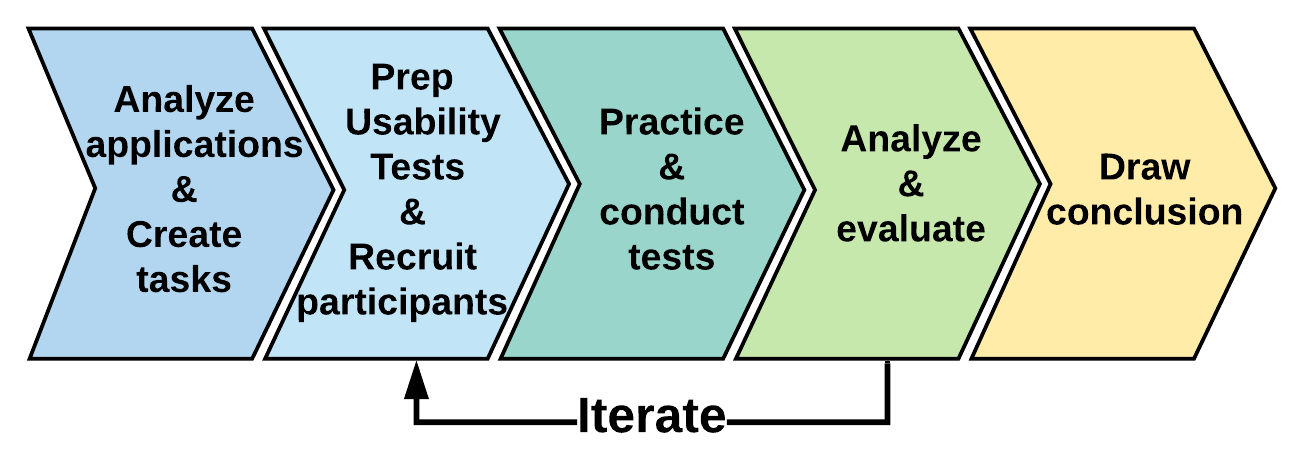
\includegraphics[width=0.9\textwidth]{img/usability_test_process.png}
	\hfill
	\caption{\textit{Process of performing a usability test}}
\end{figure}

\subsection{Multi-Criteria Decision-Method}

Several MCDM models could have been applied to this project. WSM was chosen due to its simplicity when dealing with several criteria containing dependencies. Since the WSM demands quantitative data, all qualitative data gathered was translated into quantitative data. 
Application usage was researched with an online survey, producing quantified data. \\
For the tests, quantification was done with surveys and questionnaires where test subjects quantified their own experience with the application, in combination with analyzed facial expressions and behaviour from the recordings. 
The criteria were based on input from results of our test and survey, scientific articles, software development websites and discussions with consultants at Slagkryssaren AB. \\
When a set of criteria was decided, scores were given to each alternative development tool in the model. The scores were set based on previous background research. These scores were presented to the consultants at Slagkryssaren AB and were iteratively improved upon based on their feedback. \\
When scores were set for the alternatives, the next iterative phase began. 
Use cases were run through the model, and the result was assessed. If the outcome was seen as unreasonable or unlikely to be chosen, the scores and criteria were reassessed. This iterative process was to be repeated until reasonable results are acquired, or until there was no more time to reiterate. 
